\chapter{REFERENCIAL TEÓRICO}
Para o entendimento e progresso deste trabalho, faz-se necessária a compreensão de conceitos relacionados a 
Séries Temporais, incluindo suas técnicas e modelagem, fontes de Dados Meteorológicos, 
aplicações de séries temporais em Meteorologia, redes neurais e séries temporais com redes neurais. 

\section{Séries Temporais}
    Muitas pessoas, em algum momento, já imaginaram como seria prever o futuro e ter acesso a informações sobre eventos 
    ou situações de suas vidas. Essa curiosidade reflete um desejo universal, mas também uma necessidade presente em 
    diversas áreas, como na gestão governamental, no setor financeiro e em contextos sociais. Nesse cenário, surge o 
    conceito de Série Temporal, definido como um conjunto de observações organizadas sequencialmente no tempo, 
    representadas por \( x_t \), com cada valor correspondente a um instante específico \(t\) \cite{box2015}. O estudo de 
    Séries Temporais permite não apenas compreender as características de fenômenos que evoluem ao longo do tempo, mas 
    também desenvolver e ajustar modelos estatísticos capazes de explicar ou prever o comportamento dos dados 
    observados.
    
    De acordo com~\cite{brockwell2002}, séries temporais podem ser classificadas 
    discretas e continuas, uma série temporal é discreta quando o conjunto \( t_0 \) de tempos em que as observações 
    são feitas é um conjunto discreto, como o caso de observações que são realizadas em um determinado intervalo de 
    tempo fixo. Sendo denotada por:
    \begin{equation}
        \{X_t : t \in T\}, \quad T = \{t_1, \dots, t_n\}
    \end{equation}
    
    
    
    E seríes temporais continuas quando suas observações são obtidas continualmente 
    no tempo. 
    \begin{equation}
        \{X(t) : t \in T\}, \quad T = \{t : t_1 < t < t_2\}
    \end{equation}
        

    
    Ao iniciar a análise de uma série temporal é de alta valia utilizar de gráficos criados sequencialmente no tempo,
    visto que isso pode revelar determinados padrões de comportamento e algumas características que podem estar 
    presentes nos dados, como tendência, sazonalidade, ciclidade e ruído também chamado de erro aleatório~\cite{costa2019}. 

    \subsection{Decomposição}

        A tendência ($\mu_t$) é falar o que é a tendência \\
        
        A ciclidade ($\psi_t$) pode ser \\
        
        A sazonalidade ($\gamma_t$) pode ser \\
        
        O ruído ($\epsilon_t$) é 

        %mostrar fórmula



\section{Redes Neurais}
%Falar brevemente
    O cérebro humano é um computador de grande complexidade, não linear e paralelo, 
    composto por cerca de 10 bilhões de neurônios, cada um conectado com outros 10 
    bilhões de neurônios. Em sua composição existe o corpo da célula também chamado de 
    soma, e canais da saída e entrada (dendritos e axônios) que conectam os neurônios, 
    dendritos também são chamadas zonas receptivas e axônios de linhas de transmissão. 
    Cada neurônico recebe informações eletroquimicas de outros neurônios nos dendritos 
    através dos axônios. Se as somas dessas entradas elétricas for suficientemente forte 
    para ativar o neurônio, um sinal eletroquímico ao longo do axônio, possuindo a 
    habilidade de organizar os neurônios, um dos seus componentes integradores, para 
    assim realizar várias formas de processamento de forma mais rápida que os 
    computadores digitivas convencionais~\cite{haykin2009neural}.

    A Figura \ref{fig:celula_piramidial} mostra a estrutura do neurônio:
    \begin{figure}[!htb]
        \centering
        \caption{Célula piramidial.}
        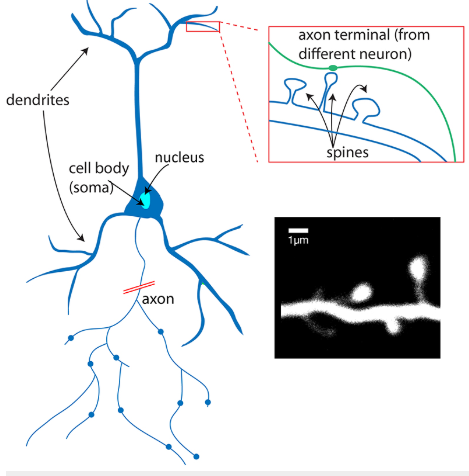
\includegraphics[scale=0.5]{celula-piramidial.png}\\
        {\footnotesize Fonte: The University Of Queensland.}\
        \label{fig:celula_piramidial}
    \end{figure}
        
    \subsection{Histórico}
        As redes neurais são frequentemente consideradas um complemento à computação tradicional. Curiosamente, 
        John von Neumann, amplamente reconhecido como o pai da computação moderna devido à sua proposta da arquitetura 
        que possibilitou a criação do computador de programa armazenado, demonstrava grande interesse em modelar o 
        funcionamento do cérebro humano. Esse interesse levantou debates entre pesquisadores sobre a possível interação 
        entre as ideias de von Neumann e os primórdios das redes neurais. Alguns estudiosos destacam indícios que 
        sugerem a visão de von Neumann sobre as direções futuras do desenvolvimento dos computadores~\cite{Fausett1994}.

        \subsubsection{Perceptrons}
            
            Em 1958, o psicólogo Frank Rosenblatt publicou um artigo que, pela primeira vez, descreveu de forma 
            algorítmica o funcionamento de um modelo de rede neural para aprendizagem supervisioanda. Essa 
            publicação inspirou inúmeros pesquisadores a direcionarem seus esforços para estudos sobre redes neurais, 
            explorando diversos aspectos dessa temática ao longo das décadas de 1960 e 1970~\cite{haykin2009neural}.

            \begin{figure}[!htb]
                \centering
                \caption{Fluxo do perceptron.}
                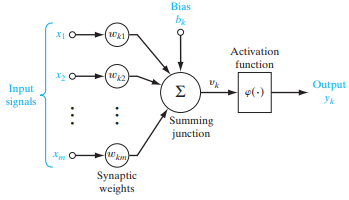
\includegraphics[scale=0.8]{fluxo-perceptron.png}\\
                {\footnotesize Fonte: Haykin (2009).}\
                \label{fig:fluxo-perceptron}
            \end{figure}

            Como apresentado na Figura~\ref{fig:fluxo-perceptron}, o perceptron consiste de um único neurônio com 
            pesos sinápticos ajustáveis e um viés. Ele possui uma camada de entrada (a retina) conectada aos pesos e 
            uma camada de saída. Seu funcionamento baseia-se em um combinador linear seguido por uma função de 
            ativação que realiza uma função linear. Esse nó somador (o neurônio) calcula uma combinação linear das 
            entradas aplicadas às suas sinapses, além de incorporar um viés aplicado externamente que ajusta a posição
            da função de ativação. O resultado dessa soma é passado à função de ativação, que produz uma saída de +1 
            se a entrada for positiva, ou -1, se for negativa. O perceptron é um classificador binário, pois resolve 
            apenas problemas de classificação de padrões linearmente separáveis, ou seja, é capaz de lidar 
            exclusivamente com problemas nos quais duas classes podem ser separadas por uma 
            linha em um hiperplano~\cite{haykin2009neural}.


        \subsubsection{Adaline}

            Em 1960, Bernard Widrow e Marcian Hoff desenvolveram uma regra de aprendizagem denominada "Regra Delta", 
            também conhecida como Least Mean Squares (LMS) ou método do Gradiente Descendente. Com base nessa regra, 
            foi criada uma rede neural com a mesma estrutura do Perceptron, composta por uma camada de entrada, uma 
            camada de saída e um único neurônio. A diferença principal residia na regra de aprendizado empregada para 
            o ajuste dos pesos.
            
            A Regra Delta, que tem como finalidade ajustar os pesos do neurônio, busca minimizar a diferença entre a 
            saída desejada e a resposta obtida a partir da combinação linear de todas as amostras. Utilizando a 
            minimização do erro quadrático médio entre os valores previstos e reais, o método opera dentro de um 
            contexto de aprendizagem supervisionada, onde há uma saída esperada previamente definida. O algoritmo 
            ajusta iterativamente o vetor de pesos \( w\) atribuído à rede, com o objetivo de determinar um 
            \( w^{*} \) ótimo tal que o erro quadrático \({E(w{*})}\), calculado sobre todo o conjunto de amostras, 
            seja minimizado.

            Essa rede neural foi projetada para aplicações em sistemas de chaveamento de circuitos telefônicos e 
            ficou conhecida como Adaline (Adaptive Linear Neuron). A Adaline foi uma das primeiras redes neurais 
            implementadas em contextos industriais, marcando um avanço significativo na aplicação de tecnologias 
            baseadas em inteligência artificial. Além disso, a regra de aprendizagem Widrow-Hoff para uma rede neural 
            de apenas uma camada foi o percursor da regra de Backpropagation para múltiplas camadas~\cite{Fausett1994,silva2010}
        \subsubsection{Backpropagation}
      
            FALAR COMO A BACKPROPAGATION FEZ AS REDES NEURAIS EVOLUIREM E VOLTAREM A SEREM ESTUDADAS
    \subsection{Componentes das Redes Neurais}
        %

    \subsection{Aprendizado em Redes Neurais}
    \subsection{Arquitetura}
    %Falar o que é e botar uma imagem em todas
        \subsubsection{Feed-Forward}
        \subsubsection{Multi Layer Perceptron}
        \subsubsection{Redes Neurais Recorrentes}
        \subsubsection{Redes Neurais Convolucionais}
        \subsubsection{Long Short-Term Memory (LSTM)}


%Talvez por na metodologia
\section{Dados Meteorológicos}

    Para a aplicação de modelos de previsão, é essencial dispor de uma quantidade significativa de dados para o 
    treinamento, validação e teste do modelo, bem como para a inferência dessas informações sobre a população como um 
    todo. No Brasil, o Instituto Nacional de Meteorologia (INMET) é o órgão responsável pelo Banco de Dados 
    Meteorológicos (BDMEP), planejado para coletar, armazenar, processar e disponibilizar dados e informações sobre 
    variáveis meteorológicas. 
    
    Esses dados podem ser gerados localmente, por meio de estações meteorológicas convencionais ou automáticas, 
    ou captados remotamente, utilizando sensores orbitais, radares, entre outros dispositivos~\cite{vianna2017}. 
    O Banco de Dados Meteorológicos para Ensino e Pesquisa (BDMEP), em particular, reúne informações meteorológicas 
    diárias provenientes das estações da rede do INMET, seguindo as normas técnicas da Organização Meteorológica 
    Mundial (INMET, s.d.).